\documentclass[tikz,border=10pt]{standalone}
\usepackage{tikz}
\usetikzlibrary{angles,quotes,animations}

\begin{document}

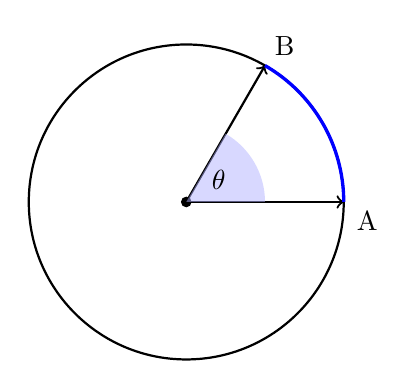
\begin{tikzpicture}[scale=2]
    % Draw the circle
    \draw[thick] (0,0) circle (1);
    
    % Mark the center
    \filldraw[black] (0,0) circle (0.03);
    
    % Draw the radius to A
    \draw[thick,->] (0,0) -- (1,0) coordinate (A);
    
    % Draw the radius to B
    \draw[thick,->] (0,0) -- ({cos(60)},{sin(60)}) coordinate (B);
    
    % Fill the smaller pie slice
    \fill[blue!30,opacity=0.5] 
        (0.5,0) -- (0,0) -- ({0.5*cos(60)},{0.5*sin(60)}) 
        arc [start angle=60, end angle=0, radius=0.5] -- cycle;
    
    % Draw the arc for the angle
    \draw[very thick,blue] (1,0) arc [start angle=0, end angle=60, radius=1];
    
    % Label the angle, adjusted to avoid overlap
    \node[above right] at (0.1,0.02) {$\theta$};
    
    % Add the points A and B
    \node[below] at (1.15,0) {A};
    \node[above right] at ({cos(60)},{sin(60)}) {B};
\end{tikzpicture}

\end{document}
